\documentclass[10pt,a4paper]{article}
\usepackage[utf8]{inputenc}
\usepackage{amsmath}
\usepackage{amsfonts}
\usepackage{amssymb}
\usepackage{graphicx}
\usepackage{enumerate}
\begin{document}
%Zack: Pages 6,7,8,19,20

%Jack: 21, 9, 10, 11

%Koka: Pages 13, 13A, 22 ,22A, 22B


\section{Generate $\mathbb{N}$}


%Ruth: Pages L4A-L4G




\section{From $\mathbb{Z}$ to $\mathbb{R}$ via ordering}
%Jazz: ZR1-ZR5

%Kyler: ZR6 - ZR10

%Preethika: ZR11-ZR14


\section{Sequence and Limits}

%Aaron: First 2 pages and 48-50

%Hamza: 51-52B

\section{Limit and Convergence}

%Joe: 50-51

%Quinten: 52-53

%Farishta: 53A-54A

\section{Infinite Series}

%Sukhreet: IS1 - IS 7

%Matthew: IS8 - IS15

%Will: IS16 - IS23

%Rebecca: IS24 - IS32

%Maady: IS33 - IS42

\section{Metric Spaces Part 1}

%Travis: M1 - M5

%Jerome: M6- M10



\section{Metric Spaces Part 2} 


%Bryant: M1-M7

Def: Let $m$ be non-empty set a metric $d$ on $m$ is a map
\newline
$d: m \times m \rightarrow$ [0,$\infty$)
\newline
satisfying (for all $x,y,z$ in $m$)
\newline
(i) $d(x,y)=d(y,x)$
$\begin{cases}
>0 \mbox{ if } x \neq y \\
=0 \mbox { if } x=y \\
\end{cases}$
\newline
(ii) $d(x,y)\leq d(x,z)+d(z,y)$
\newline
(iii) is called the triangle ineq
\newline
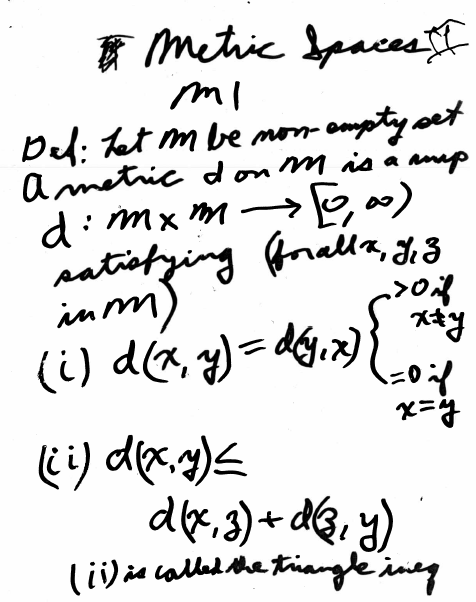
\includegraphics[scale=.5]{Pages/MS_2_im1}
\newpage
\underline{Examples}
\newline
1. $d(x,y) =$
$\begin{cases}
\mbox { 1 } if x \neq y \\
\mbox { 0 } if x = y
\end{cases}$
\newline
2. If $m=R^k$ and $1\leq P$ $\leq \infty$
\newline
$d_p$($\vec{x}$,$\vec{y}) = (\sum_{j=1}^{k} (x_j-y_j)^p)^\frac{1}{p}$
\newline
$d_\infty(\vec{x},\vec{y}) = max_{1\leq j \leq k} |x_j-y_j|$
\newline
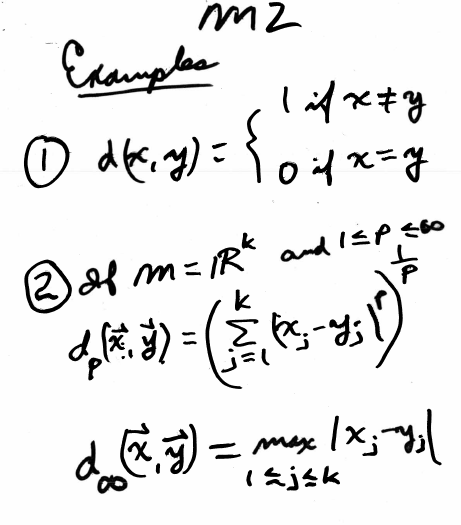
\includegraphics[scale=.5]{Pages/MS_2_im2}
\newpage
New Metrics From Old
\newline
Suppose $d(x,y)$ is a metric 
\newline
on $m$ and $f$:[0,$\infty$)$\rightarrow$ [0,$\infty$) is non-decreasing with 
\newline
$f$(0)=0 and $f(x)>$0 if $x>$0.
\newline
When will
\newline
$g(x,y)=f(d(x,y))$ be a metric?
\newline
We need to guarantee that the triangle inequality holds for $g$.
\newline
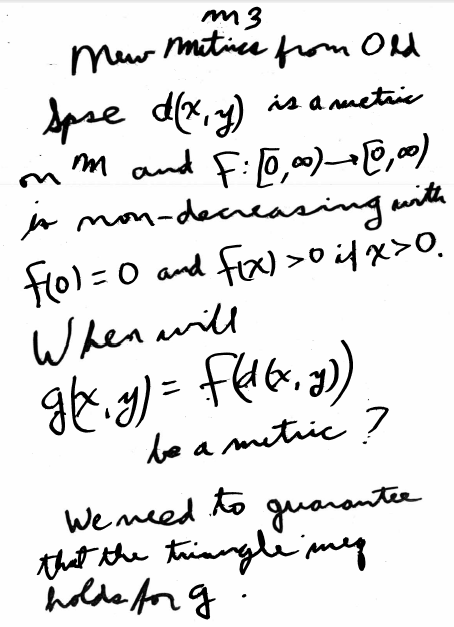
\includegraphics[scale=.5]{Pages/MS_2_im3}
\newpage
Suppose $f(a+b)\leq f(a)+f(b)$
\newline
for $a\geq$0, $b\geq$ 0 (Then $f$ is sub-additive)
\newline 
then
\newline
$g(x,y)=f(d(x,y))$
\newline
$\leq f(d(x,z)+d(z,y))$
\newline
$\leq f(d(x,z))+f(d(z,y))$
\newline
$=g(x,z)+g(z,y)$
\newline
If $f'(y) \geq$ 0 and $f ''(y)\leq$ 0 and $f(0)$ = 0 then $f$ is sub-additive
\newline
ex. $f(y)=\sqrt{y}$
\newline
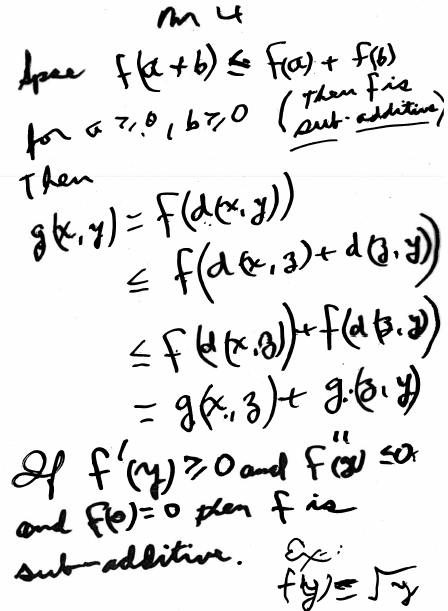
\includegraphics[scale=.5]{Pages/MS_2_im4}
\newpage
If $d_1$ and $d_2$ are metrics on m then
\newline
$d(x,y)=\max \{ d_1(x,y),d_2(x,y) \}$ may not be a metric, but
\newline
$\min \{ d(x,y),1 \}$ is a metric
\newline
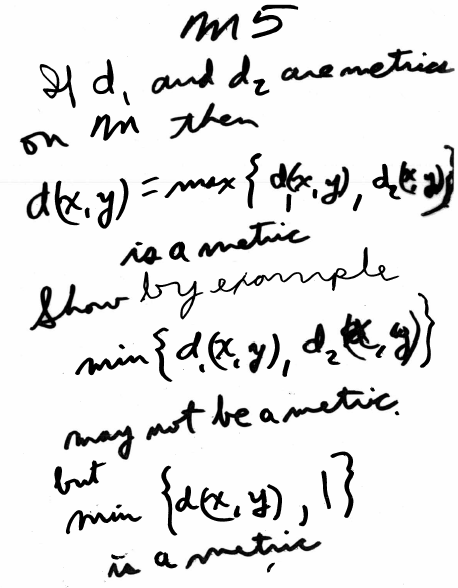
\includegraphics[scale=.5]{Pages/MS_2_im5}
\newpage
An Aside: why do mathematicians call virtually every non-empty set a $\underline{space}$?
\newline
$\underline{Answer}$:The $\underline{space}$ we inhabit can be represented by the $\underline{set}$ of ordered triples $(x_1,x_2,x_3)$ of reals. Hence we think of a way non-empty set as an abstract space.
\newline
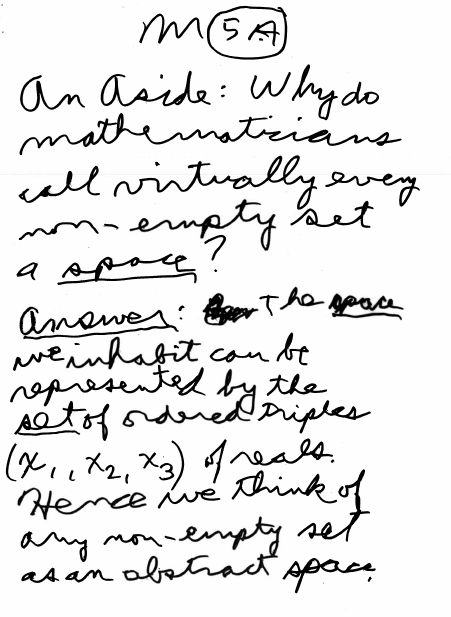
\includegraphics[scale=.5]{Pages/MS_2_im6}
\newpage
$\underline{Convergence of a Sequence}$
\newline
Let $x, x_n \in m$ Then $x_n \rightarrow x$ in $m$ in metric $d$ 
\newline
if
\newline
$\forall$ $\epsilon$ $\geq$ 0 $\exists N_\epsilon < \infty$
\newline
such that
\newline
$d(x_n,x)< \epsilon$
\newline
for all $n \geq N_\epsilon$ 
\newline
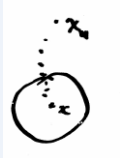
\includegraphics[scale=1]{Pages/MS_2_pic1}
\newline
$\underline{Fact 1}$. Limits are unique
\newline
Proof: Suppose $x_n \rightarrow x$ and $x_n \rightarrow y$
\newline
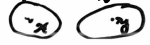
\includegraphics[scale=1]{Pages/MS_2_pic2}
\newline
How can $x_n$ be in both sets
\newline
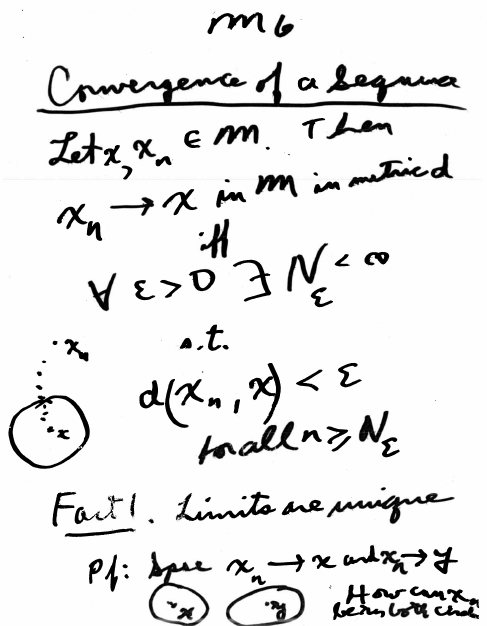
\includegraphics[scale=.5]{Pages/MS_2_im7}
\newpage
\underline{Subsequent Limits}
\newline
Given \{ $a_n$ \}, let $\mathcal{L}$= \{ susequential limits \}
\newline
Can we upper bound $\mathcal{L}$
\newline
Let
$b_1$= suppose $\{ a_1,a_2,... \}$
\newline
$b_2$= suppose $\{ a_2,a_3,... \}$
\newline
$b_n$= suppose $\{ a_n,a_{n+1},... \}$
\newline
$b_1 \geq b_2 \geq ...$
\newline
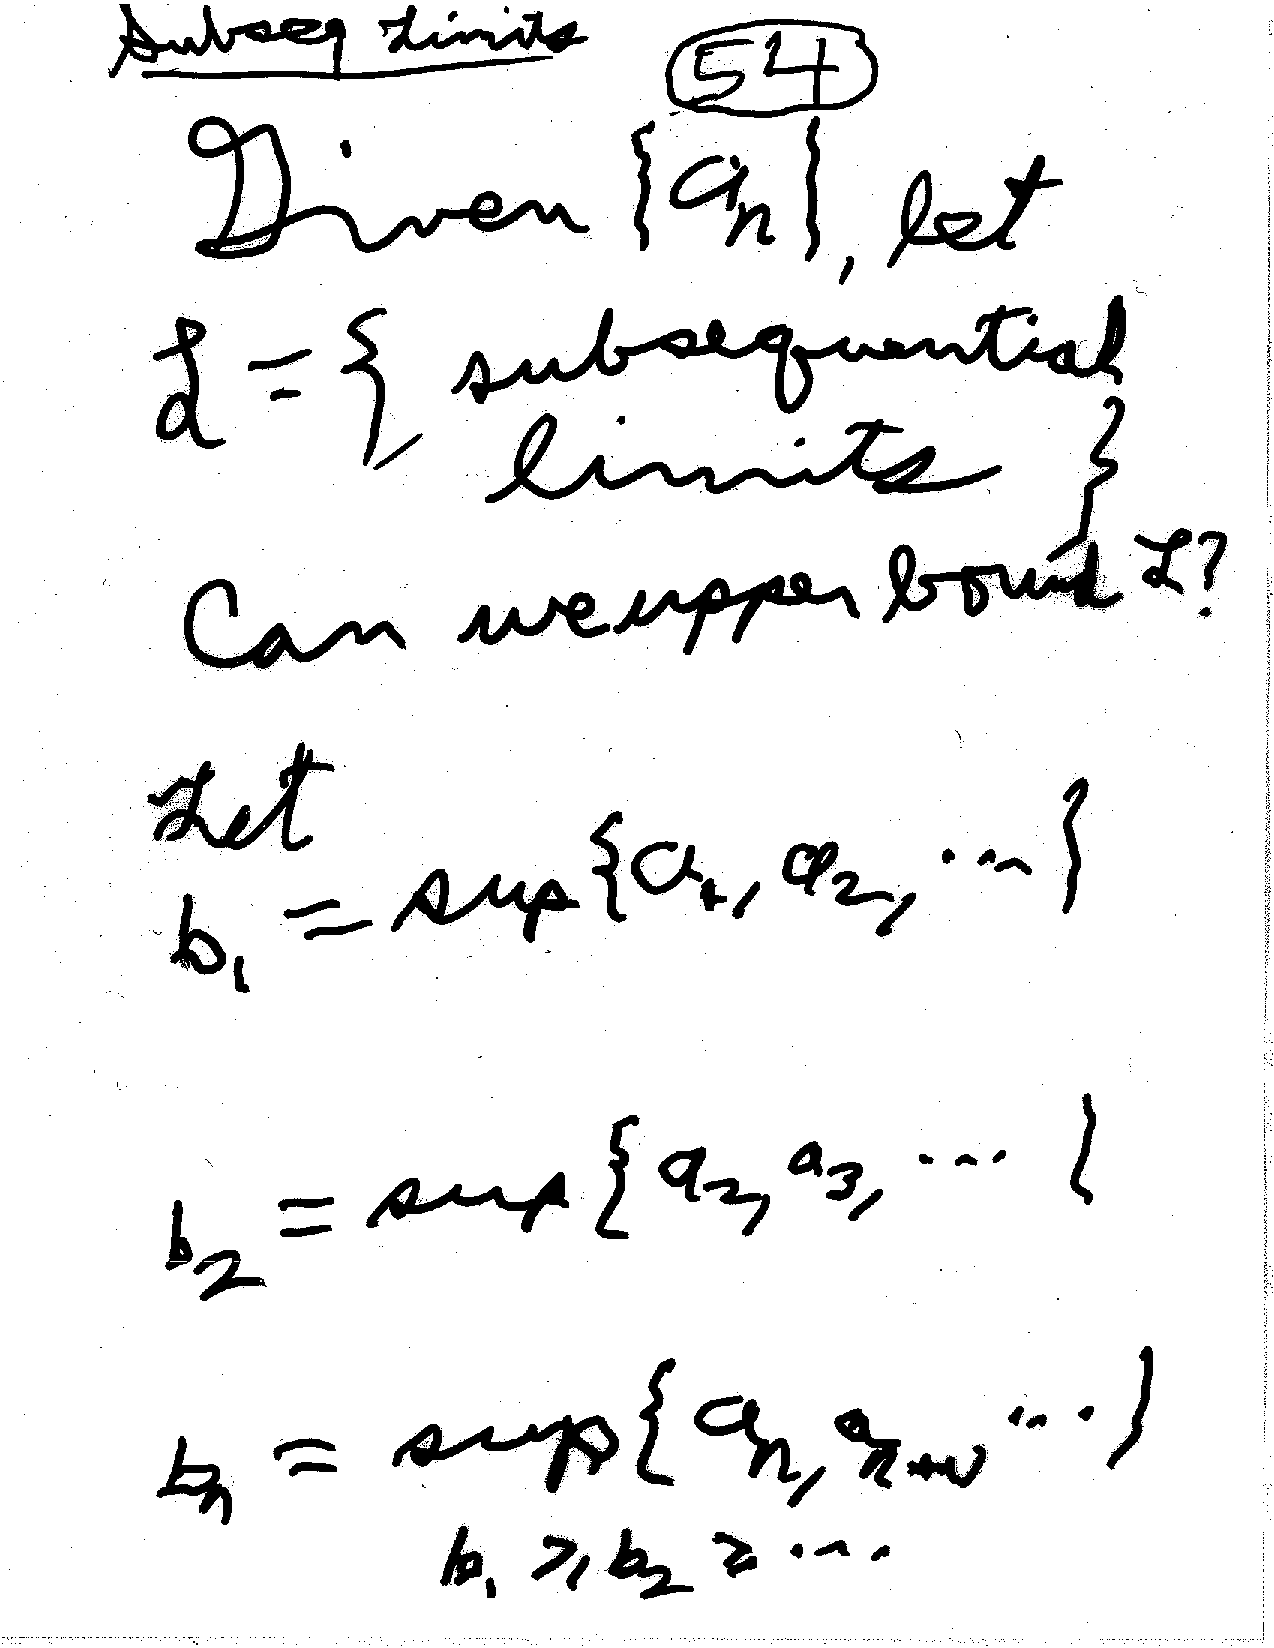
\includegraphics[scale=.5]{Pages/LC_1}
\newpage
Definition: $$\limsup_{n \rightarrow \infty} a_n = \lim_{n \rightarrow \infty} b_n$$
\newline
$$\equiv \lim_{n\rightarrow \infty} [\sup (a_k : k\geq n)]
= \inf_{n} [\sup (a_k -k > n)]$$
\newline
Clearly,
\newline
$$\sup \mathcal{L} \leq \lim_{n \rightarrow \infty} a_n$$
\newline
Can you show they are equal?
\newline
What about $\inf$ $\mathcal{L}$?
\newline
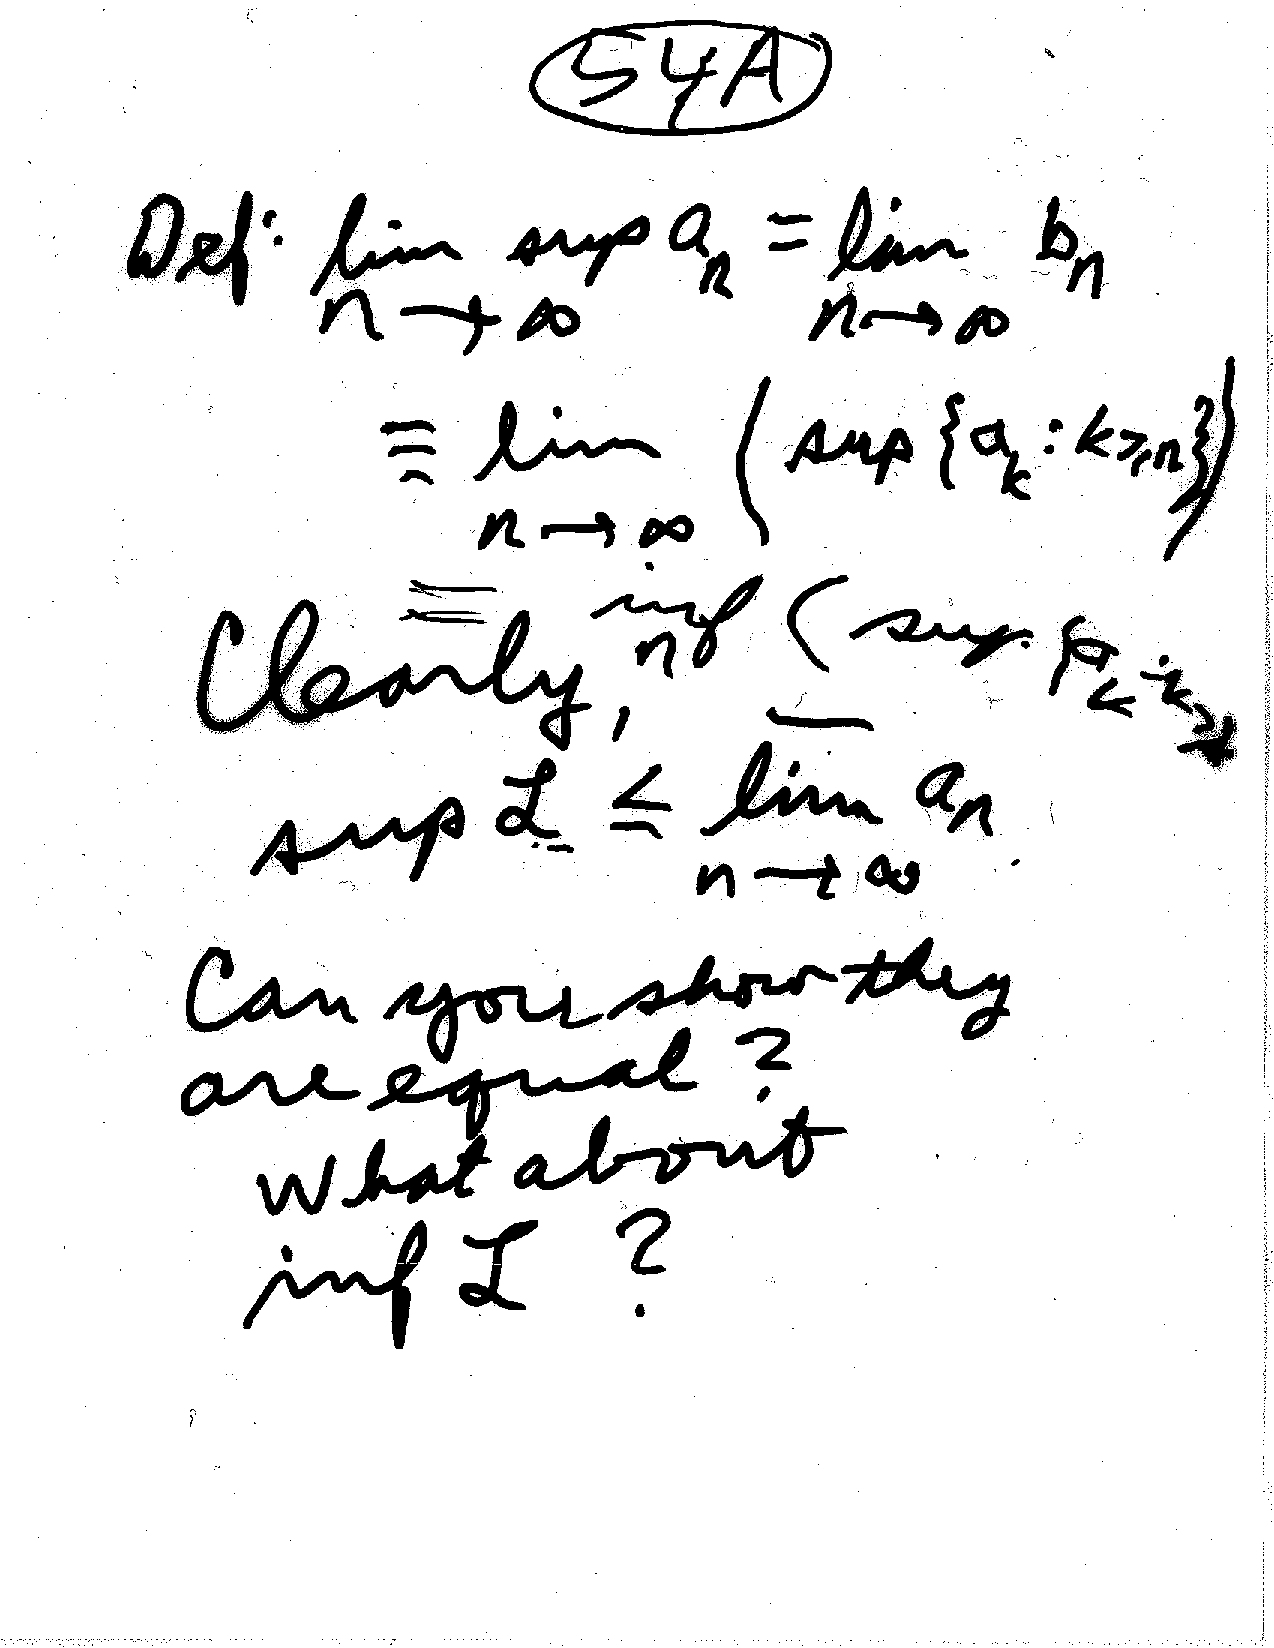
\includegraphics[scale=.4]{Pages/LC_2}



%Reshma: M8-M14

%Ethan: M15-M21





\end{document}